We now consider ablation studies to better identify the best positional embedding, activation function, and embedding normalization placement. 

\subsection{Positional Embeddings}

\begin{table}[b]
\begin{center}
\begin{tabular}{@{}cc@{}}
\toprule
\textbf{Positional Embedding} & \textbf{Average EAI Results}\\
\midrule
None & 41.23\\
Learned & 41.71\\
Rotary & 41.46\\
ALiBi & \textbf{43.70} \\ 
\bottomrule
\end{tabular}
\end{center}
\caption{\textbf{ALiBi significantly outperforms other embeddings for zero-shot generalization.} All models are trained on the OSCAR dataset for 112 billion tokens.}
\label{tab:positional}
\end{table}

\paragraph{Background} Originally, both static sinusoidal position embeddings and learned position embeddings were proposed to capture positionnal information; the latter are popular in large language models \cite{brown2020gpt3}. 
\citet{su2021roformer} proposed rotary embeddings, where the query and key representations inside the self-attention mechanism are modified such that the attention captures relative distances between them. Recently, \citet{press2021alibi} introduced a method which does not use embeddings, instead directly attenuating the attention scores based on how far away the keys/queries are. 

\paragraph{Results} We compare learned, rotary, and ALiBi position embeddings, and include a baseline without position embeddings. Our results are presented in Table~\ref{tab:positional}. Although learned positional embeddings outperform rotary embeddings, ALiBi yields significantly better results than all alternatives. We also confirm the findings of~\citet{biderman2021nopos}: a baseline with no positional information exhibits competitive performance. While bidirectional models require positional embeddings to determine the location of tokens, we find autoregressive models can simply leverage the causal attention mask. We also confirm the ability of ALiBi to extrapolate to longer sequences than trained on in Figure \ref{fig:extrapolation}. Note that results in Table~\ref{tab:positional} do not use any extrapolation: ALiBi embeddings are a better choice even without taking into account their ability to extrapolate. 

\begin{figure}[h]
    \centering
    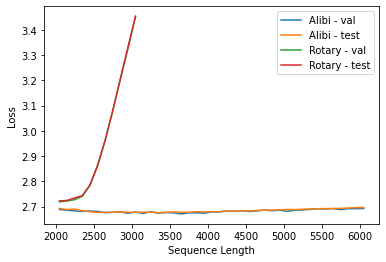
\includegraphics[width=\columnwidth]{figures/extrapolation.png}
    \caption{\textbf{ALiBi embeddings can effectively extrapolate past the sequence length on which the model was trained, while rotary embeddings can not.} This is in line with the findings of \citet{press2021alibi}.}
    \label{fig:extrapolation}
\end{figure}

\begin{table}[b]
\begin{center}
\begin{tabular}{@{}cc@{}}
\toprule
\textbf{Activation function} & \textbf{Average EAI Results}\\
\midrule
GELU & 42.79\\
SwiGLU & \textbf{42.95}\\
\bottomrule
\end{tabular}
\end{center}
\caption{\textbf{SwiGLU slightly outperforms GELU for zero-shot generalization.} Models trained on The Pile for 112 billion tokens.}
\label{tab:activation}
\end{table}

\begin{mdframed}
\textbf{Finding 2.} ALiBi positional embeddings significantly outperforms other embeddings for zero-shot generalization.
\end{mdframed}


\subsection{Activation Functions}

\paragraph{Background.} Large language models by and large still mostly use the GELU activation \cite{hendrycks2016gaussian}. We evaluate a recently proposed alternative, SwiGLU \cite{shazeer2020swiglu}, which combines both Gated Linear Units \cite{dauphin2016glu} with the Swish activation function \cite{ramachandran2017searching}. 

SwiGLU uses $50\% $ extra parameters in the feed-forward layers. As suggested in \citet{shazeer2020swiglu}, we compensate for this by reducing the hidden size of the feed-forward layer. 

\paragraph{Results.} We present our results in Table~\ref{tab:activation}. SwiGLU produces slightly better results than GELU. For our final model, we adopted GELU, as we initially observed a lower throughput for SwiGLU. However, further benchmarking identified that this overhead was primarily associated with the change in the hidden size of the feedforward network. Indeed, this new size, 5,456, is divisible by neither the warp size of the GPU~\citep{Lashgar2013WarpSI} nor the number of streaming multiprocessors, resulting in both tile and wave quantization. We accordingly recommend using SwiGLU for future models.


\subsection{Embedding Norm}

\citet{bitsandbytes} suggests that greater stability of training can be achieved by including an extra layer normalization \cite{layernorm} after the embedding layer. We evaluate the performance impact of such a modification in Table~\ref{tab:emb_norm}. We note that this incurs a significant reduction in the performance of the model. However, models above 100 billion parameters are notoriously unstable and require considerable engineering efforts in order to be kept stable. If this addition provides increased stability when training, it may be valuable. 


\begin{table}[b]
\begin{center}
\begin{tabular}{@{}cc@{}}
\toprule
\textbf{Embedding Norm} & \textbf{Average EAI Results}\\
\midrule
No & \textbf{43.46}\\
Yes &  42.24\\
\bottomrule
\end{tabular}
\end{center}
\caption{\textbf{Layer normalization after the embedding layer diminishes performance significantly.} Models trained on The Pile for 300 billion tokens.}
\label{tab:emb_norm}
\end{table}

\begin{mdframed}
\textbf{Finding 3.} Adding layer normalization after the embedding layer incurs a significant penalty on zero-shot generalization. 
\end{mdframed}
